\documentclass{beamer}
\usepackage{beamerthemeshadow}
\usepackage{color}
\usepackage{graphicx}
%\usepackage[all]{xy}

%\newcommand{\allcomments}[1]{{#1}}
%\definecolor{JoesGold}{RGB}{204,102,0}
%\definecolor{ForestGreen}{RGB}{34,139,34}
%\newcommand{\joecomment}[1]{{\bf \color{JoesGold}{\allcomments{{#1}}}}}
%\newcommand{\elenacomment}[1]{{\bf \textcolor{ForestGreen}{\allcomments{{#1}}}}}

\mode<presentation>
{
  \usetheme{Copenhagen} %%% Change later
 \usecolortheme{beaver}


  \setbeamercovered{transparent}
  % or whatever (possibly just delete it)
}
\setbeamertemplate{footline}[page number]{}


\begin{document}
\title{Static vs Dynamic Types in Software Development}
\author{Emma Callery}
\institute[UMM] % (optional, but mostly needed)
{
 % \inst{1}%
  University of Minnesota, Morris
}
\date[May 13, 2013]  
{UMN Morris Senior Seminar Conference Fall 2014}

\begin{frame}
  \titlepage
\end{frame}

\begin{frame}
	\frametitle{Outline}
\tableofcontents
\end{frame}

\section{Static and Dynamic Types}
\begin{frame}
	\frametitle{Static Types}
	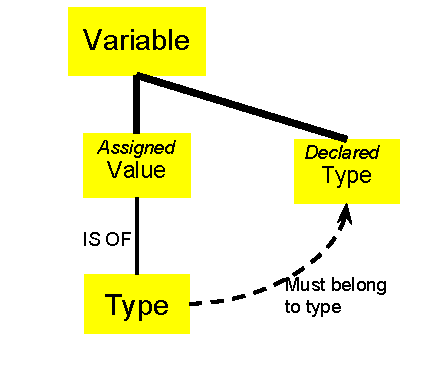
\includegraphics{Static_Type_Diagram}
\end{frame}
\begin{frame}
	\frametitle{Dynamic Types}
	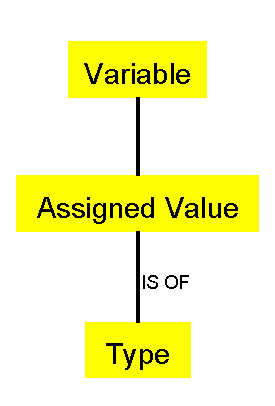
\includegraphics{Dynamic_Type_Diagram}
\end{frame}

\section{How Programmers use Types}
\begin{frame}
	\frametitle{Study of Programmer Preferences}
		6638 Open Source Groovy projects were analyzed to try to determine 'in which contexts Groovy programmers type or do not type their declarations' to answer five proposed questions on the behavior of programmers.
\end{frame}
\begin{frame}
	\frametitle{Study Questions}
	\begin{itemize}
	\item[Q 1] Do programmers use types more often in the
interface of their modules?
	\item[Q 2]Do programmers use types less often in test
classes and scripts?
	\item[Q 3]Does the experience of programmers with
other languages influence their choice for typing their code?
	\item[Q 4]Does the experience of programmers with
other languages influence their choice for typing their code?
	\item[Q 5]In frequently changed code, do developers
prefer typed or untyped declarations?
	\end{itemize}
\end{frame}
\begin{frame}
	\frametitle{Analysis}
	
\end{frame}
\begin{frame}
	\frametitle{Results}
\end{frame}
	
\section{Influence of Static Types}
\begin{frame}
	\frametitle{Study of the Influence of Static Types on Usability}
\end{frame}
\begin{frame}
	\frametitle{Results}
\end{frame}
	
\section{Type Systems and Development Time}
\begin{frame}
	\frametitle{Study on the Relationship Between Type Casts and Development Time}
\end{frame}
\begin{frame}
	\frametitle{Results}
\end{frame}
	
\section{Conclusions}
\begin{frame}
	\frametitle{Conclusion}
\end{frame}

\end{document}

